
\pagebreak
\subsection{\stmt{SVERWEIS}}


$$ \text{\stmt{SVERWEIS( \syntax{Suchkriterium}; \syntax{Matrix}; \syntax{Spaltenindex}; [\syntax{Bereichsverweis}]} )}$$
Diese Funktion ist eine Art Kombination aus \stmt{VERGLEICH} und \stmt{INDEX} in der Matrixversion. Sie sucht ähnlich wie \stmt{VERGLEICH} innerhalb einer Spalte einen Suchwert und gibt aus einer Matrix den Wert im Schnittpunkt der so gefundenen Zeile mit einer eingegebenen Spaltenzahl zurück.



\begin{description}[labelindent=0cm, leftmargin=3.5cm, font=\mdseries, labelwidth=3.5cm,style=nextline]
\item[\syntax{Suchkriterium}] Dieser Wert wird in der in der ersten Spalte, also die sich ganz links befindet, der Suchmatrix gesucht. Genauso wie bei der \stmt{VERGLEICH} Funktion gibt es einen \stmt{\#NV} Fehler, wenn der Suchwert kleiner als der kleinste Wert in der Suchspalte ist.
\item[\syntax{Matrix}] Ein Zellbezug von mindestens zwei Spalten
\item[\syntax{Spaltenindex}] Eine Ganzzahl, welche jene Spalte der Matrix angibt, deren Wert zurückgegeben werden soll. Wenn eine Spalte < 1 gewählt wird, gibt es den Fehler \stmt{\#Wert!}, ist die gewünschte Spalte größer als die Spaltenzahl der Matrix, dann gibt es einen Fehler \stmt{\#Bezug!}.
\item[\syntax{Bereichsverweis}] %
	\begin{description}[labelindent=0cm, leftmargin=3cm, font=\mdseries, labelwidth=3cm,style=nextline]
	\item[\stmt{WAHR} (default)] Sucht nach dem größtem Wert, der kleiner oder gleich dem Suchkriterium ist. Die erste Spalte der Suchmatrix muss aufsteigend sortiert sein.
	\item[\stmt{FALSCH}] Sucht eine genaue ÜBereinstummung. Hier muss die erste Spalte der Matrix \textit{nicht} sortiert sein.
	\end{description}


\end{description}

Nehmen wir an, dass Kunden auf Grund ihrer Umsätze am Ende des Jahres einen Rabatt bekommt. Es wird also für jeden Kunden einzeln in der Rabatttabelle, welche hier die Matrix ist, nachgesehen, welchen Rabatt der Kunde bekommt. 

\pagebreak
	\begin{figure}[H]
		\centering
%			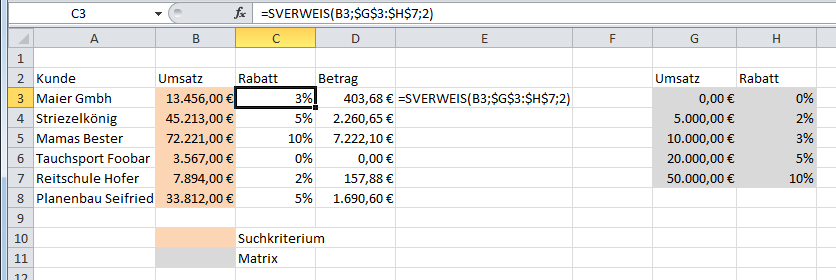
\includegraphics[width=12cm]{images/sverweis_b}
			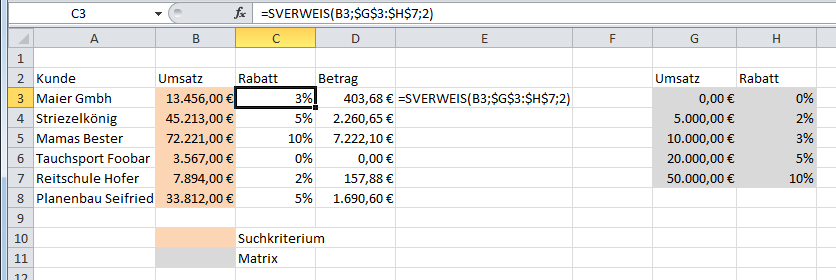
\includegraphics[scale=0.7]{images/sverweis_b}
		\caption{\stmt{SVERWEIS} zur Rabattfindung}
		\label{fig:sverweis}
	\end{figure}
Bei der Reitschule Hofer beträgt der Jahresumsatz 7.894 Euro. Dieser Wert wird herangezogen, um in der Umsatzspalte der Matrix, dem Bereich \xlc{F3:G7}, die Zeile zu finden die größer gleich dem Wert in der Zeile, aber kleiner als der Wert in der nächsten Zeile ist. 7.894 ist größer als 5.000, aber kleiner als 10.000. Daher ist diese Zeile die gesuchte. Nun wollen wir nur den Wert aus der zweiten Spalte, die ja den Rabattbetrag festlegt.




\begin{lightbulbbox}
Man kann sich die Funktion des \stmt{SVERWEIS} ganz einfach durch "`Was suche ich wo und die wievielte Spalte will ich als Ergebnis haben."' merken.
\end{lightbulbbox}


\begin{lightbulbbox}
Beim Verwenden von \stmt{SVERWEIS} wird gerne übersehen, dass man den Matrixbereich in der Formel fixieren sollte. Also statt \xlc{F4:G7} sollte \xlc{\$F\$4:\$G\$7} verwendet werden. Dadurch wird der Matrixbereich beim Kopieren der Formel in andere Zellen nicht verändert.
\end{lightbulbbox}


\subsection{\stmt{WVERWEIS}}


Der \stmt{WVERWEIS} funktioniert genauso wie der \stmt{SVERWEIS}, nur dass die Matrix nicht zeilenorientiert, sondern spaltenorientiert augebaut ist.


$$ \text{\stmt{SVERWEIS( \syntax{Suchkriterium}; \syntax{Matrix}; \syntax{Zeilenindex}; [\syntax{Bereichsverweis}]} )}$$

Das Beispiel aus dem Abschnitt mit dem \stmt{SVERWEIS} würde also so aussehen.
	\begin{figure}[H]
		\centering
%			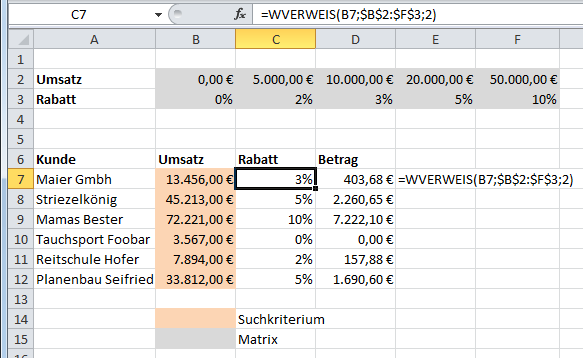
\includegraphics[width=12cm]{images/wverweis_b}
			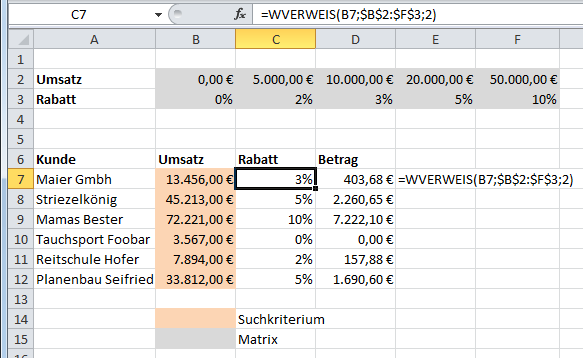
\includegraphics[scale=0.7]{images/wverweis_b}
		\caption{\stmt{WVERWEIS} zur Rabattfindung}
		\label{fig:wverweis}
	\end{figure}